For SFibAI, w/o View, w/o Weak Loc., and full VCRE-Fib, validation selects epochs 65, 80, 39, and 47, with $\risk$ of 0.172661, 0.157844, 0.159315, and 0.156067. Validation contains 20,880 images, 1,227 patients, and 33 centers. Appendix Table~\ref{tab:freeze} records the four frozen checkpoints; Figure~\ref{fig:training} shows their trajectories under the common 90-epoch cap. Test risk determines ranking; validation documents selection.
\inputtable{tab10_freeze}
The four models use four GPUs with SyncBatchNorm and global batch 24 under the common training settings in Appendix~\ref{sec:appendix-implementation}. Validation selects from epochs 21--90 by $\risk$, image COR, then earlier epoch; selected checkpoints are frozen before test evaluation. Figure~\ref{fig:training} shows all 90 recorded epochs without smoothing. Total losses contain different auxiliary terms and serve as within-model diagnostics. Figure~\ref{fig:losses} shows the full model's loss components.
\begin{figure}[!htbp]
\centering
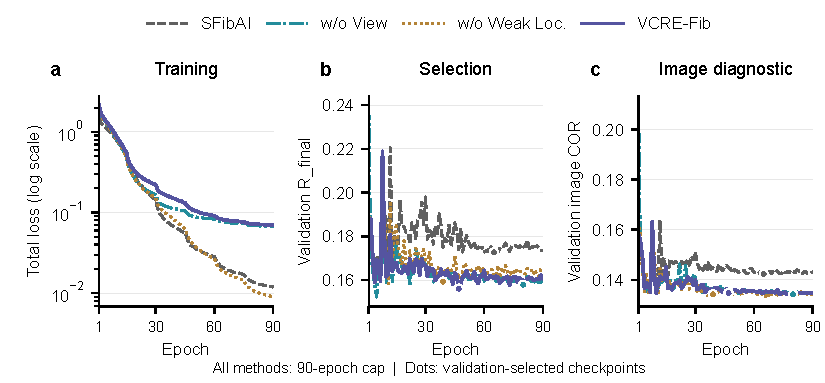
\includegraphics[width=\linewidth]{figures/assets/training_curves.pdf}
\caption{\lang{Training and validation trajectories under a common 90-epoch cap. (a) Total training loss on a logarithmic axis, including each model's auxiliary terms. (b) Validation $R_{\mathrm{final}}$. (c) Validation image COR. Curves show unsmoothed epoch-level observations; dots mark the validation-selected checkpoints in Table~\ref{tab:freeze}.}{统一 90 epoch 上限下的训练与验证集轨迹。(a) 含各模型辅助项的训练总损失，纵轴为对数尺度。(b) 验证集 $R_{\mathrm{final}}$。(c) 验证集 image COR。曲线为未经平滑的逐轮观测，圆点标记表~\ref{tab:freeze} 中由验证集选择的检查点。}}\label{fig:training}
\end{figure}

\begin{figure}[!htbp]
\centering
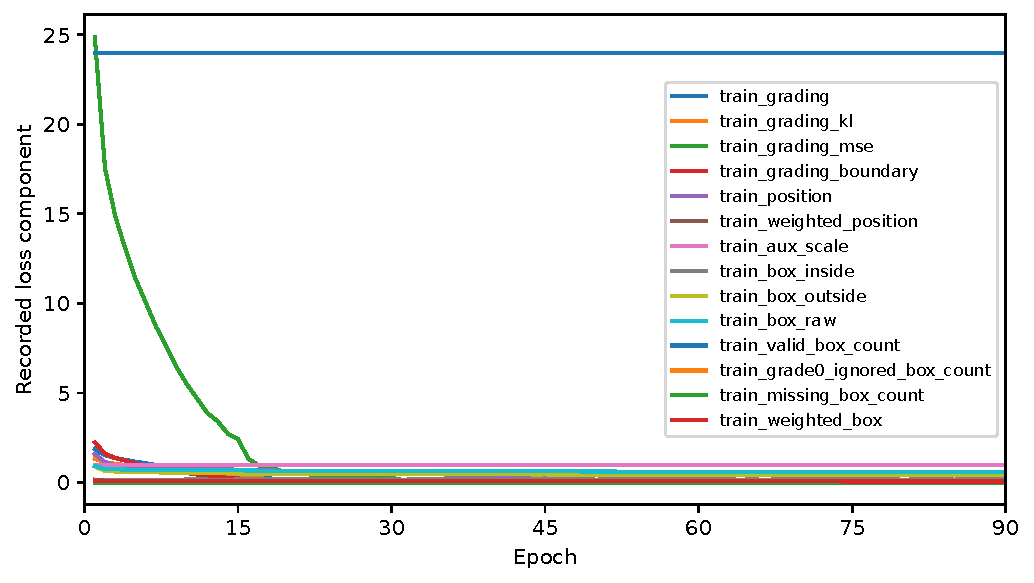
\includegraphics[width=\linewidth]{figures/assets/synap_loss_components.pdf}
\caption{\lang{Full VCRE-Fib loss components under the same 90-epoch cap, shown as training diagnostics rather than estimates of module effects.}{完整 VCRE-Fib 在相同 90 epoch 上限下的训练损失分项，用于训练诊断，不作为模块效应估计。}}\label{fig:losses}
\end{figure}

\FloatBarrier
